% This LaTeX document needs to be compiled with XeLaTeX.
\documentclass[
  10
]{article}
\usepackage[margin=2cm,includehead=true,includefoot=true,centering,]{geometry}
\usepackage{xcolor}
\usepackage{ucharclasses}
\usepackage{hyperref}
\usepackage{amsmath,amssymb}
\usepackage{amsfonts}
\usepackage[version=4]{mhchem}
\usepackage{stmaryrd}
\usepackage{bbold}
\usepackage{polyglossia}
\usepackage{fontspec}
\usepackage{ctex}
\usepackage[export]{adjustbox}
\usepackage{tabularx}
\usepackage{booktabs}

\usepackage{setspace}
\setstretch{1.2}

\makeatletter
\@ifundefined{KOMAClassName}{% if non-KOMA class
  \IfFileExists{parskip.sty}{%
    \usepackage{parskip}
  }{% else
    \setlength{\parindent}{0pt}
    \setlength{\parskip}{6pt plus 2pt minus 1pt}}
}{% if KOMA class
  \KOMAoptions{parskip=half}}
\makeatother
\usepackage{graphicx}
\makeatletter
\newsavebox\pandoc@box
\newcommand*\pandocbounded[1]{% scales image to fit in text height/width
  \sbox\pandoc@box{#1}%
  \Gscale@div\@tempa{\textheight}{\dimexpr\ht\pandoc@box+\dp\pandoc@box\relax}%
  \Gscale@div\@tempb{\linewidth}{\wd\pandoc@box}%
  \ifdim\@tempb\p@<\@tempa\p@\let\@tempa\@tempb\fi% select the smaller of both
  \ifdim\@tempa\p@<\p@\scalebox{\@tempa}{\usebox\pandoc@box}%
  \else\usebox{\pandoc@box}%
  \fi%
}
% Set default figure placement to htbp
\def\fps@figure{htbp}
\makeatother
\setlength{\emergencystretch}{3em} % prevent overfull lines
\providecommand{\tightlist}{%
  \setlength{\itemsep}{0pt}\setlength{\parskip}{0pt}}


\hypersetup{colorlinks=true, linkcolor=blue, filecolor=magenta, urlcolor=cyan,}
\urlstyle{same}

\usepackage{colortbl}
\definecolor{table-row-color}{HTML}{999999}
\definecolor{table-rule-color}{HTML}{999999}
%\arrayrulecolor{black!40}
\arrayrulecolor{table-rule-color}     % color of \toprule, \midrule, \bottomrule
\setlength{\aboverulesep}{0pt}
\setlength{\belowrulesep}{0pt}


\setotherlanguages{english}
\IfFontExistsTF{Source Han Serif CN}
{\newfontfamily\chinesefont{Source Han Serif CN}}
{\IfFontExistsTF{Noto Serif CJK SC}
  {\newfontfamily\chinesefont{Noto Serif CJK SC}}
  {\IfFontExistsTF{SimSun}
    {\newfontfamily\chinesefont{SimSun}}
    {\IfFontExistsTF{FangSong}
      {\newfontfamily\chinesefont{FangSong}}
      {\newfontfamily\chinesefont{Arial Unicode MS}}
}}}
\IfFontExistsTF{Times New Roman}
{\newfontfamily\englishfont{Times New Roman}}
{\IfFontExistsTF{Liberation Serif}
  {\newfontfamily\englishfont{Liberation Serif}}
  {\IfFontExistsTF{DejaVu Serif}
    {\newfontfamily\englishfont{DejaVu Serif}}
    {\newfontfamily\englishfont{Arial}}
}}


\author{}
\date{}

\begin{document}


\section{Stochastic computing}\label{stochastic-computing}

by B. R. GAINES

Standard Telecommunication Laboratories

Harlow, Essex, United Kingdom

\section{INTRODUCTION}\label{introduction}

The Stochastic Computer was developed as part of a program of research
on the structure, realization and application of advanced automatic
controllers in the form of Learning Machines. \(^{1,2}\) Although
algorithms for search, identification, policy-formation and the
integration of these activities, could be established and tested by
simulation on conventional digital computers, there was no hardware
available which would make construction of the complex computing
structure required in a Learning Machine feasible. The main problem was
to design an active storage element in which the stored value was stable
over long periods, could be varied by small increments, and whose output
could act as a `weight' multiplying other variables. Since large numbers
of these elements would be required in any practical system it was also
necessary that they be small and of low cost. Conventional analog
integrators and multipliers do not fulfill requirements of stability and
low cost, and unconventional elements such as electro-chemical stores
and transfluxors are unreliable or require sophisticated external
circuitry to make them usable. \(^3\) Semiconductor integrated circuits
have advantages in speed, stability, size and cost, and it was decided
to design a computing element based on standard gates and flip-flops
which would be amenable to large-scale integration.

A binary up/down counter has the properties of an incremental store, but
requires many bits if the increments are too small and of variable size.
If incrementing is made a stochastic process, however, `fractional
increments' may be effected in the stored count. Thus, if an increment
of one-tenth of the value corresponding to the least significant bit is
required, the counter may be incremented by unity with a probability of
one-tenth---this is the basic principle of stochastic computing to
represent analog quantities by the probability that an event will occur.
This principle was first embodied in the ADDIE, a smoothing and storage
device with stochastic input and output

for realization of the STeLLA learning scheme, \(^{1}\) and later
extended to give rise to a family of computing elements capable of
performing all the normal functions of an analog computer---this was
called a Stochastic Computer. \(^{4}\)

It is impossible within the scope of this paper to do more than describe
briefly a few basic stochastic computing elements and configurations;
Reference 4 discusses the theoretical basis of stochastic computing and
describes some previous uses of random variables in data-processing,
whilst Reference 5 describes the application of stochastic computing to
process identification by means of gradient techniques, Bayes estimation
and prediction, and Markov modelling.

\section{Stochastic representation of numerical
data}\label{stochastic-representation-of-numerical-data}

The stochastic computer is an incremental, or `counting,' computer whose
computations involve the interaction of unordered sequences of logic
levels (rather than digital arithmetic between binary `words'), and is
in this respect similar to the Digital Differential Analyser, \(^{6}\)
Operational Hybrid Computer, \(^{7}\) and Phase Computer. \(^{8}\) In
all these computers quantities are represented as binary words for
purposes of storage, and as the proportion of ON logic levels in a
clocked sequence (or frequency of pulses in the operational computers
and asynchronous DDAs) for purposes of computation. In conventional
computers, however, the sequences of logic levels are generated
deterministically and are generally patterned or repetitious, whereas in
the stochastic computer each logic level is generated by a statistically
independent process; only the generating probability of this process is
determined by the quantity to be represented.

This distinction is illustrated in Figure 1 which shows typical
sequences in the various forms of computer: (a) is the output from a
synchronous rate multiplier, or from the `R register' of a DDA,
corresponding to a store \(\frac{3}{4}\) full---it will be noted that
the ON and OFF logic levels are distributed as uniformly as possible;
(b) is the output of a differential

\begin{enumerate}
\def\labelenumi{(\alph{enumi})}
\tightlist
\item
  O I I O I I O I I O I I Output from Rate Multiplier\\
\item
  Output from Differential Store\\
\item
  OIOI I I I IOO I I I O\\
\item
\item
\item
  Ensemble of Stochastic Sequences
\end{enumerate}

Figure 1---Typical computing sequences in various incremental computers

store in the Phase Computer---the OFF logic levels in a cycle all occur
before the ON logic levels giving the synchronous equivalent of a
mark/space modulated signal; (c) through (f) are examples of stochastic
sequences with a generating probability of \(\frac{3}{4}\) ---any
sequence {[}including (a) and (b){]} may occur, but the proportion of ON
levels in a large sample of such sequences will have a binomial
distribution with a mean of \(\frac{3}{4}\) .

Although a probability is a continuous variable capable of representing
analog data without quantization error, this variable cannot be measured
exactly and is subject to estimation variance. The effect of this
variance on the efficiency of representation may be seen by comparing
the number of levels required by various computers to carry analog data
with a precision of one part in N:

\begin{itemize}
\tightlist
\item
  The analog computer requires one continuous level;\\
\item
  The digital computer requires log₂ kN ordered binary levels;\\
\item
  The DDA requires kN unordered binary levels; and\\
\item
  The stochastic computer requires \(\mathbf{kN}^2\) unordered binary
  levels;
\end{itemize}

where \(\mathbf{k} > 1\) is a constant representing the effects of
round-off error or variance, \(\mathbf{k} = 10\) say. The
\(\mathbf{N}^2\) term for the stochastic computer arises because the
expected error in estimating a generating probability decreases as the
square-root of the length of sequence sampled.

Although this progression from 1:
\(\log_2\mathbf{N}:\mathbf{N}:\mathbf{N}^2\) shows the stochastic
computer to be the least efficient

in its representation of quantity, the lack of coherency or patterning
in stochastic sequences enables simple hardware to be used for complex
calculations with data represented in this way.

\section{Stochastic computing}\label{stochastic-computing-1}

Although there are occasions when the {[}0, 1{]} range of probabilities
may be used directly in computation, e.g.~Bayes estimation and
prediction, it is usually necessary to map analog variables into this
range both by scaling and shift of origin. Many mappings have been
investigated, but the two considered in this paper are of particular
interest because they give rise to computations similar to those of the
conventional analog computer. These are:

\begin{enumerate}
\def\labelenumi{(\roman{enumi})}
\tightlist
\item
  Single-line symmetric representation.-Given a quantity, \(\mathbf{E}\)
  , in the range \(-\mathbf{V} \leq \mathbf{E} \leq \mathbf{V}\) ,
  represent it by a sequence with generating probability,
  \(\mathfrak{p}\) , such that:
\end{enumerate}

\[
p (O N) = \frac {1}{2} E / V + \frac {1}{2} \tag {1}
\]

so that maximum positive quantity is represented by a logic level always
ON, maximum negative quantity by its being always OFF, and zero quantity
by a random sequence with equal probability of being ON or OFF.

\begin{enumerate}
\def\labelenumi{(\roman{enumi})}
\setcounter{enumi}{1}
\tightlist
\item
  Dual-line symmetric representation.-The first representation suffers
  from the disadvantage that zero quantity is represented with maximum
  variance, and when values near zero must be distinguished it is better
  to use a two-line stochastic representation. Let the quantity,
  \(\mathbf{E}\) , in the range
  \(-\mathbf{V} \leq \mathbf{E} \leq \mathbf{V}\) , be represented by
  sequences on two lines, the UP and DOWN lines, such that:
\end{enumerate}

\[
p (U P = O N) = \left\{ \begin{array}{l l} E / V & \text {i f} E > 0 \\ 0 & \text {i f} E \leqslant 0 \end{array} \right. \tag {2}
\]

\[
p (\text {D O W N} = \text {O N}) = \left\{ \begin{array}{l l} - E / V & \text {i f} E <   0 \\ 0 & \text {i f} E \geq 0 \end{array} \right. \tag {3}
\]

These equations give a minimum variance representation which is not
necessarily maintained during a computation, and the most general form
of the Dual-Line Symmetric Representation follows from the inverse
equation:

\[
\mathrm {E} / \mathrm {V} = \mathrm {p} (\mathrm {U P} = \mathrm {O N}) - \mathrm {p} (\mathrm {D O W N} = \mathrm {O N}) \tag {4}
\]

The next sections describe stochastic computing elements to perform the
complete range of analog computing functions, inversion, multiplication,
addition, integration, and so on, using synchronous logic elements
acting on stochastic sequences.

\section{Stochastic invertors, multipliers and
isolators}\label{stochastic-invertors-multipliers-and-isolators}

To multiply a quantity in representation (ii) by \(-1\) requires only
the interchange of UP and DOWN lines. In representation (i) the logical
inverter, whose output is the complement of its input, performs the

same function. Consider the relationship between the probability that
its output will be ON, \(\mathbf{p}^{\prime}\) , and the

\pandocbounded{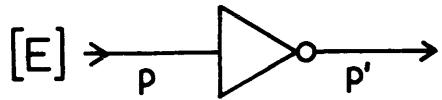
\includegraphics[keepaspectratio]{images/18d7613076ce6b0b84df55368587204853773f3bf1656c71baec0bb9c0de0068.jpg}}\\
(i)

\pandocbounded{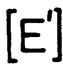
\includegraphics[keepaspectratio]{images/a7e3dde6defc4d322291b683a51c20141404cb8e8c32ef9fd37ff00d0fba7c72.jpg}}

\pandocbounded{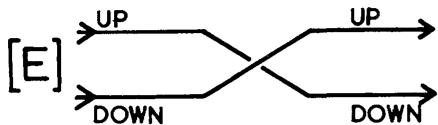
\includegraphics[keepaspectratio]{images/68c65ca36123c3d82fddcaf1df05b677ad33b03343b3eb9d9fff753353cca733.jpg}}\\
(ii)

\pandocbounded{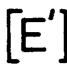
\includegraphics[keepaspectratio]{images/86ba6abc9fda47b79c62b862d02370849d7f831e54829cc3bf2f281b7179cb60.jpg}}\\
Figure 2---Stochastic invertors

probability that its input will be ON, p; that is

\[
p ^ {\prime} = 1 - p \tag {5}
\]

From equation (1), the relationship between these probabilities and the
quantities they represent is:

\[
\begin{array}{l} p = \frac {1}{2} E / V + \frac {1}{2} (6) \\ p ^ {\prime} = \frac {1}{2} E ^ {\prime} / V + \frac {1}{2} (7) \\ \end{array}
\]

hence

\[
\mathbf {E} ^ {\prime} = - \mathbf {E} \tag {8}
\]

Multiplication of one quantity by another may be effected by an inverted
exclusive-OR gate in representation (i), and by a pair of similar gates
in representation (ii); realizations of these stochastic multipliers in
NAND logic are shown in Figures 3(i) and 3(ii) respectively.

\pandocbounded{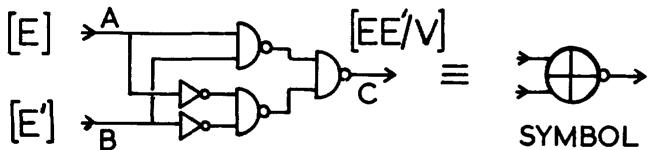
\includegraphics[keepaspectratio]{images/006cd21d90ed91a778330bc2c7410063641a619aaeebcfebb6a1829dec084b21.jpg}}\\
(i) \(C = A.B \vee \overline{A}.\overline{B}\)

\pandocbounded{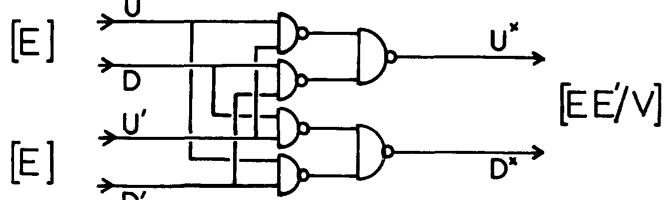
\includegraphics[keepaspectratio]{images/87b5233b7b2642581fc555b9961d8e8aaeb4f0652acf86b532de3129ae1a8def.jpg}}\\
U= U.Uv D.D' (ii)\\
D*= U.D'v D.U'\\
Figure 3---Stochastic multipliers

That multiplication does occur may be confirmed by examination of the
relationship between input and output probabilities for the gates of
Figure 3. For 3(i) we have:

\[
\begin{array}{l} \mathrm {p} (\mathrm {C}) = \mathrm {p} (\mathrm {A}) \mathrm {p} (\mathrm {B}) + (1 - \mathrm {p} (\mathrm {A})) (1 - \mathrm {p} (\mathrm {B})) \\ \text {a n d f r o m e q u a t i o n (1) : -} \end{array} \tag {9}
\]

\[
p (A) = \frac {1}{2} E / V + \frac {1}{2} \tag {10}
\]

\[
p (B) = \frac {1}{2} E ^ {\prime} / V + \frac {1}{2} \tag {11}
\]

so that:

\[
p (C) = \frac {1}{2} \left(E E ^ {\prime} / V\right) / V + \frac {1}{2} \tag {12}
\]

which is normalized multiplication of E by \(\mathbf{E}^{\prime}\) .A
similar result is obtained for 3(ii) by substitution from equation (4)
in the relationships:-

\[
\begin{array}{l} p (U ^ {*}) = p (U) p \left(U ^ {\prime}\right) + p (D) p \left(D ^ {\prime}\right) - \tag {13} \\ \mathrm {p} (\mathrm {U . U ^ {\prime} . D . D ^ {\prime}}) \\ \end{array}
\]

and:

\[
\begin{array}{r l} \mathrm {p} (\mathrm {D} ^ {\mathrm {x}}) & = \mathrm {p} (\mathrm {U}) \mathrm {p} (\mathrm {D} ^ {\prime}) + \mathrm {p} (\mathrm {D}) \mathrm {p} (\mathrm {U} ^ {\prime}) - \\ & \mathrm {p} (\mathrm {U}. \mathrm {U} ^ {\prime}. \mathrm {D}. \mathrm {D} ^ {\prime}) \end{array} \tag {14}
\]

An important phenomenon is illustrated by the use of a stochastic
multiplier as a squarer. For example, it is not sufficient to
short-circuit the inputs of the gate in Figure 3(i), for its output will
then be always ON. This difficulty arises because we have assumed that
the stochastic input sequences are statistically independent in
obtaining equation (9) above. Fortunately an independent replication of
a stochastic sequence (in fact a Bernoulli sequence) may be obtained by
delaying it through one event, and Figure (4) illustrates how a squarer
may be constructed using the multiplier of Figure 3(i) together with a
flip-flop used as a delay; similarly the multiplier of Figure 3(ii) may
be used as a squarer by feeding delayed replicas of U and D to U' and D'
respectively. Flip-flops used in this way act as stochastic `isolators',
performing no computation but statistically isolating two
cross-correlated lines.

\pandocbounded{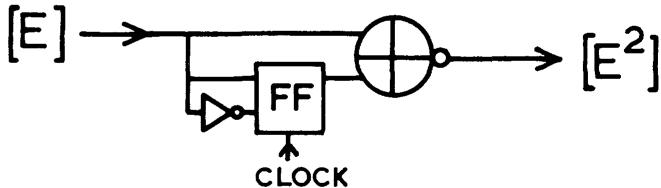
\includegraphics[keepaspectratio]{images/879c30ec366d098fb9151a70770fff6be90fbcfc2bb7c014fac61ebfe974c207.jpg}}\\
Figure 4---Stochastic squarer

\section{Stochastic summers}\label{stochastic-summers}

Having seen how readily inversion and multiplication may be performed by
simple gates, one is tempted to assume that similar gates may be used to
perform addition. However this is not so, and stochastic logic elements
must be introduced to sum the quantities represented by two stochastic
sequences. For example, consider two stochastic sequences in
representation (i), one representing maximum positive quantity and hence
always ON, the other representing maximum negative quantity and hence
always OFF. The sum of these quantities is zero, and this is represented
by a stochastic sequence with equal probabilities of being ON or OFF. A
probabilistic output cannot be obtained

from a deterministic gate with constant inputs, so that stochastic
behaviour must be built into the summing gates of a stochastic computer.

Stochastic summers may be regarded as switches which, at a clock-pulse,
randomly select one of the input lines and connect it to the output. The
output line then represents the sum of the quantities represented by the
input lines, weighted according to the probability that a particular
input line will be selected. The random selection is performed by
internally-generated stochastic sequences, obtained either by sampling
flip-flops triggered by a high bandwidth noise source, or from a delayed
sequence of a central pseudo-random shift-register; these sequences we
call `digital noise.'

\pandocbounded{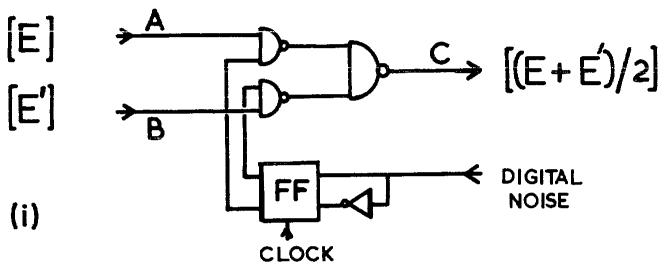
\includegraphics[keepaspectratio]{images/5dc94beb4b8df8ffaa7d0969fa68d04c38fcfc80f4ba37c1f9038e19a6ebcd10.jpg}}

\pandocbounded{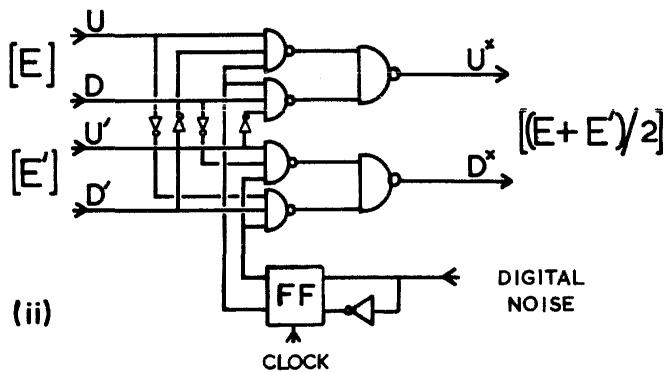
\includegraphics[keepaspectratio]{images/bbed31d4771fbde4344e3774419967d9fc2a2d9dec06eb85f04836fb0862bd0f.jpg}}\\
Figure 5---Stochastic summers

Two-input stochastic summers for quantities in representations (i) and
(ii) are shown in Figures 5(i) and 5(ii) respectively; the
cross-coupling between the inputs in Figure 5(ii) reduces the variance
of the output. That addition does occur may be confirmed by examination
of the relationship between input and output probabilities for the gates
of Figure 5. For 5(i), assuming symmetrically distributed digital noise,
we have:

\[
\mathbf {p} (\mathrm {C}) = \frac {1}{2} \mathbf {p} (\mathrm {A}) + \frac {1}{2} \mathbf {p} (\mathrm {B}) \tag {15}
\]

and hence from equations (10) and (11):---

\[
\mathbf {p} (\mathbf {C}) = \frac {1}{2} \left(\frac {1}{2} \left(\mathrm {E} + \mathrm {E} ^ {\prime}\right)\right) / \mathrm {V} + \frac {1}{2} \tag {16}
\]

which is normalized summation of \(\mathbf{E}\) and
\(\mathbf{E}^{\prime}\) . A similar result is obtained for 5(ii) by
substitution from equation (4) in the relationships:

\[
\begin{array}{l} p (U ^ {x}) = \frac {1}{2} p (U) (1 - p (D ^ {\prime})) + \frac {1}{2} p (U ^ {\prime}) \\ (1 - \mathbf {p} (D)) \tag {17} \\ \end{array}
\]

\[
\begin{array}{l} p \left(\mathrm {D} ^ {\mathrm {x}}\right) = 1 / 2 p (\mathrm {D}) (1 - p \left(\mathrm {U} ^ {\prime}\right)) + 1 / 2 p \left(\mathrm {D} ^ {\prime}\right) \\ (1 - p (U)) \tag {18} \\ \end{array}
\]

Stochastic integrators, the ADDIE and interface

The basic integrator in a stochastic computer is a reversible
counter---if this has \(\mathbf{N} + 1\) states, then the value of the
integral when it is its k'th state is:

\[
f = (2 k / N - 1) V \tag {19}
\]

If this quantity is to be used in further computations it must be made
available as a stochastic sequence, and this may be generated by
comparing the binary number in the counter with a uniformly distributed,
digital random number (obtained from a central pseudo-random
shift-register or a sampled cycling counter). In representation (i) the
integrator output line is ON if the stored-count is greater than the
random number. In representation (ii) the stored count is regarded as a
number in twos-complement notation, whose magnitude is compared with the
random number, and whose sign together with the result of this
comparison determines whether the UP or DOWN output lines shall be ON.

\pandocbounded{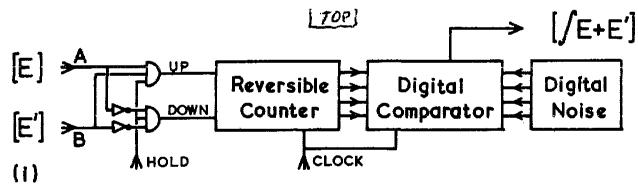
\includegraphics[keepaspectratio]{images/007a2e69d1cdef90fea0e84ae3f7f572dd8e39f1a4ab896936ec0d15e7299444.jpg}}

\pandocbounded{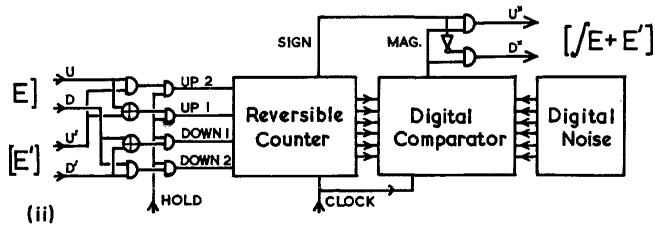
\includegraphics[keepaspectratio]{images/16ec18facc1380b8aa3b7486b50e51a35cfe61959404adde710f746e5c26117d.jpg}}\\
Figure 6---Stochastic integrators

Figure 6 shows two-input stochastic integrators for each representation
with output lines as described above, and gating at the input of the
counters to form the sum of the quantities represented by the input
lines (stochastic summing is not required because the number of lines
used to represent the sum is greater than the number of lines used to
represent each input). A HOLD line at the input of the integrators
determines whether they are in the integrate or hold modes, and

the normal integrator symbol is used for the overall device as shown in
Figure 7.

\pandocbounded{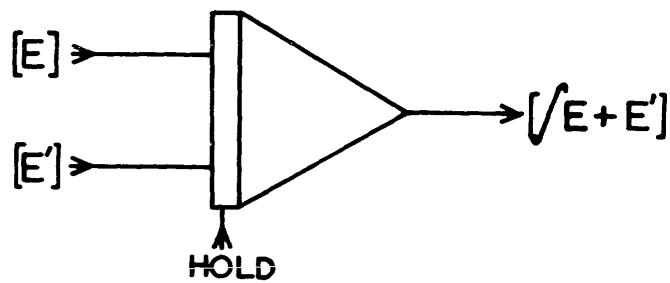
\includegraphics[keepaspectratio]{images/75a79ae91e0524d8a4a085913776e7eb6366e36494880280cd89973d641fcbec.jpg}}\\
Figure 7---Integrator symbol

That integration does occur may be confirmed by examination of the
expected increment, \(\delta\) , in the counter at each clock-pulse. For
6(i):

\[
\begin{array}{l} \delta = \frac {2 \mathrm {V}}{\mathrm {N}} [ \mathrm {p} (\mathrm {A}) \mathrm {p} (\mathrm {B}) - (1 - \mathrm {p} (\mathrm {A}) (1 - \mathrm {p} (\mathrm {B})) ] (20) \\ = \left(\mathrm {E} + \mathrm {E} ^ {\prime}\right) / \mathrm {N} (21) \\ \end{array}
\]

by substitution from equations (10) and (11), which is equivalent to an
integrator with a time-constant:

\[
\mathrm {T} = \mathrm {N} / \mathrm {f} \tag {22}
\]

where \(f\) is the clock-frequency. A similar result may be obtained for
6(ii) by substituting from equation (4) in the relationship:

\[
\begin{array}{l} \delta = \frac {2 \mathrm {V}}{\mathrm {N}} [ 2 \mathrm {p} (\mathrm {U}) \mathrm {p} (\mathrm {U} ^ {\prime}) + \mathrm {p} (\mathrm {U}) (1 - \mathrm {p} (\mathrm {U} ^ {\prime})) + \mathrm {p} (\mathrm {U} ^ {\prime}) \\ (1 - p (U)) - 2 p (D) p \left(D ^ {\prime}\right) - p (D) (1 - p \left(D ^ {\prime}\right)) \\ - p (D ^ {\prime}) (1 - p (D)) ] (23) \\ = \frac {2 V}{N} [ p (U) - p (D) + p \left(U ^ {\prime}\right) - p \left(D ^ {\prime}\right) ] (24) \\ = 2 \left(\mathrm {E} + \mathrm {E} ^ {\prime}\right) / \mathrm {N} (25) \\ \end{array}
\]

which is equivalent to integration with a time constant:

\[
\mathrm {T} = \mathrm {N} / 2 \mathrm {f} \tag {26}
\]

where \(f\) is the clock-frequency.

\pandocbounded{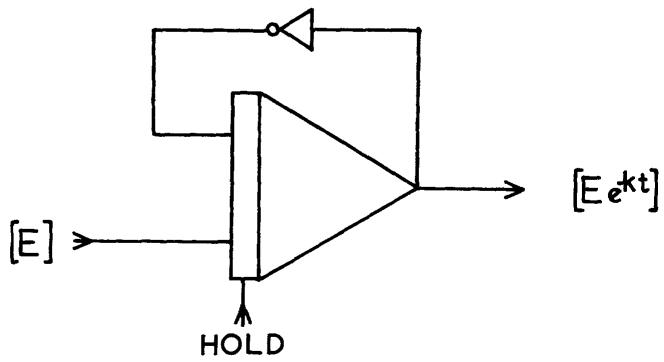
\includegraphics[keepaspectratio]{images/0cdd3c8d1eaae3776bcc0f46af2de49d369be1891bdabfe0bafb2233add619e1.jpg}}\\
Figure 8-ADDIE

The integrator with unity feedback illustrated in Figure 8 is called an
ADDIE, and performs the important function of exponentially averaging
the quantity represented by its input. In terms of the quantity
represented it may be regarded as a transfer function: \(1 / (s + 1)\) ,
and in terms of the stochastic sequences

it may be shown that the fractional count in the store tends to an
unbiased estimate of the probability that the input line will be ON at a
clock-pulse (for the integrator of Figure 6(i) connected as in Figure
8). That is, for an \(\mathbf{N} + 1\) state store in its \(k^{\prime}\)
th state:

\[
\hat {\mathbf {p}} (\text {I N P U T} = \mathrm {O N}) = \mathrm {k} / \mathrm {N} \tag {27}
\]

with an estimation time of order N clock-pulses, and a final variance:

\[
\sigma^ {2} (\hat {\mathfrak {p}}) = \mathrm {p} (1 - \mathrm {p}) / \mathrm {N} \tag {28}
\]

Thus any quantity represented linearly by a probability in the
stochastic computer may be read out to any required accuracy by using an
ADDIE with a sufficient number of states, but the more states the longer
the time-constant of smoothing and the lower the bandwidth of the
computer. Since the distribution of the count in the integrator is
binomial, and hence approximately normal for large N, variables within
the stochastic computer may be regarded as degraded by Gaussian noise
whose power increases in proportion to the bandwidth required from the
computer.

Integrators or ADDIEs form the natural output interface of the
stochastic computer. Integrators with their HOLD lines OFF also form the
input interface for digital or analog data, since binary numbers may be
transferred directly into the counter to generate a stochastic output
sequence, and analog quantities may be converted to binary form by
comparison with a standard ramp generated by a cycling counter driving a
digital/analog converter. Similarly an integrator may be used to hold a
constant and thus act as a `potentiometer' if coupled to a multiplier.
Arbitrary functional relationships may be realized by imposing a
suitable nonlinear relationship between the stored count and the
stochastic output; for example, an integrator whose output is ON when
the count is equal to or above mid-value, and OFF when it is below
mid-value {[}in representation (i){]} approximates to a switching
function.

\pandocbounded{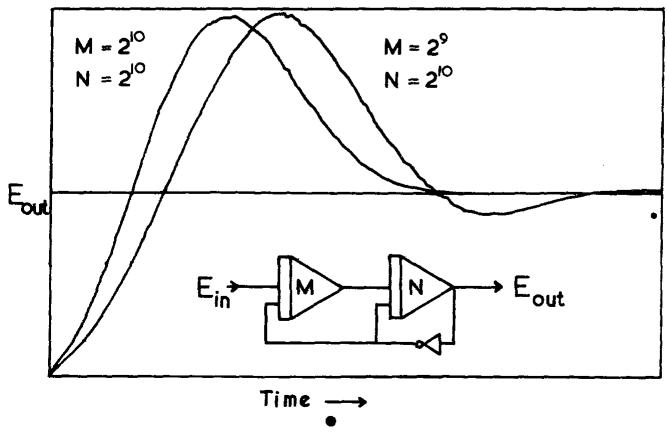
\includegraphics[keepaspectratio]{images/ed44eb7f2d5c2d711785ea2583ca50f72f6b7b5057c9faad71f2c99fcd1d2e5f.jpg}}\\
Figure 9---Stochastic second order transfer function---response to unit
step in position and velocity

Higher-order smoothing than that of the ADDIE may be realized by
connecting integrators in cascade with appropriate feedback loops. The
inset of Figure 9 shows a stable second-order stochastic
transfer-function using two stochastic integrators in representation
(i). If the first integrator has \(\mathbf{M} + 1\) states, and the
second \(\mathbf{N} + 1\) , then the transformation realized is:

\[
\frac {\mathrm {M N}}{\mathrm {f} ^ {2}} \mathrm {E} _ {\text {o u t}} + \frac {\mathrm {M}}{\mathrm {f}} \mathrm {E} _ {\text {o u t}} + \mathrm {E} _ {\text {o u t}} = \mathrm {E} _ {\text {i n}} \tag {29}
\]

where \(f\) is the clock-frequency. So that the undamped natural
frequency is:

\[
\mathrm {f} _ {\mathrm {n}} = \frac {\mathrm {f}}{2 \Pi (\mathrm {M N}) ^ {1 / 2}} \tag {30}
\]

and the damping ratio is:

\[
\Sigma = 1 / 2 (\mathrm {M} / \mathrm {N}) ^ {1 / 2} \tag {31}
\]

The responses to unit step in position and velocity for the two
conditions: \(\mathbf{M} = 2^{10}\) , \(\mathbf{N} = 2^{10}\) and
\(\mathbf{M} = 2^{9}\) , \(\mathbf{N} = 2^{10}\) : are shown in Figure
9; these were obtained on the Mark I Stochastic Computer at STL.

\section{Generation of stochastic
sequences}\label{generation-of-stochastic-sequences}

The central problem in constructing a stochastic computer is the
generation of many stochastic sequences (K for each integrator, where K
is the number of flip-flops in the integrator counter), which are
neither cross-correlated nor autocorrelated, and which have known,
stable generating probabilities. This reduces to a requirement for a
number of independent sequences each with a generating probability of
\(\frac{1}{2}\) , since any probability may be expressed as a fractional
binary number and realized to any required accuracy by appropriate
gating of a set of lines equally likely to be ON or OFF. For example,
Figure 10 illustrates one technique for generating stochastic sequences
with a generating probability of \(\frac{1}{2}\) by sampling flip-flops
toggling rapidly from a noise source: the following NAND gates convert
two of these sequences to one with a generating probability of
\(\frac{3}{4}\) . This may be confirmed from the relationship:

\[
\mathrm {p} (\mathrm {C}) = (1 - \mathrm {p} (\mathrm {A})) + \mathrm {p} (\mathrm {A}) \mathrm {p} (\mathrm {B}) = 3 / 4 \tag {32}
\]

The generation of digital noise as shown in Figure 10 is quite
attractive since radio-active or photon-emitting sources may be coupled
directly to semiconductor devices to form random pulse generators. It
suffers from the disadvantage that very high toggling rates must be
attained in \(\mathbf{F}\mathbf{F}_1\) and
\(\mathbf{F}\mathbf{F}_1^{\prime}\) and sampled by very narrow strobes
in \(\mathbf{F}\mathbf{F}_2\) and \(\mathbf{F}\mathbf{F}_2^{\prime}\) ,
if a high clock-frequency is to be used.

The Mark I Stochastic Computer had six ten-bit integrators, each with
their own internal digital noise source consisting of ten-bit counters
cycling at a high clock-frequency. These counters were sampled at a very
much lower and anharmonic clock-frequency to

\pandocbounded{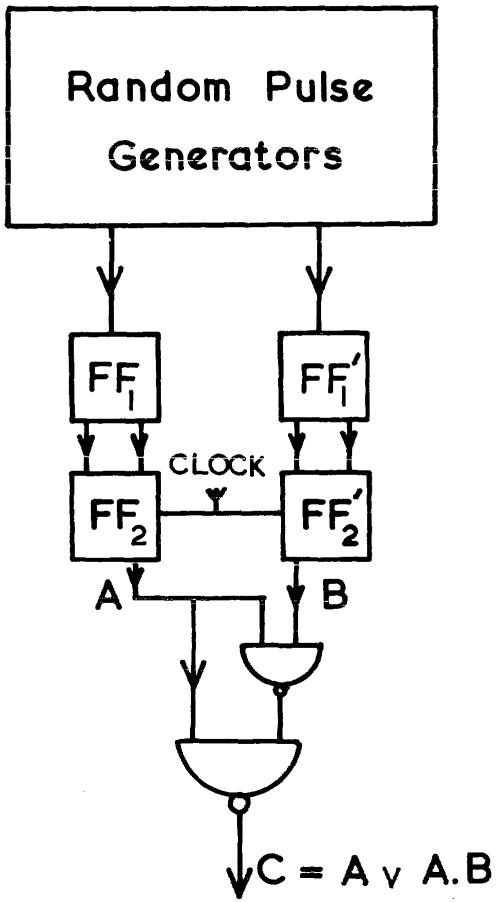
\includegraphics[keepaspectratio]{images/86d4c25b150612ffb31e1017b90576a3917bdbf1872594a8388c5304573a1f6b.jpg}}\\
Figure 10---Generation of stochastic sequence \((p = 3/4)\)

give an effectively random output. This was not a practical arrangement
since the sampling frequency had to be so low (500 cs), that the overall
bandwidth of the computer was only 0·1 cs !; as an experimental tool,
however, it has enabled us to check out configurations, such as that of
Figure 9, whose behaviour is difficult to determine theoretically.

\pandocbounded{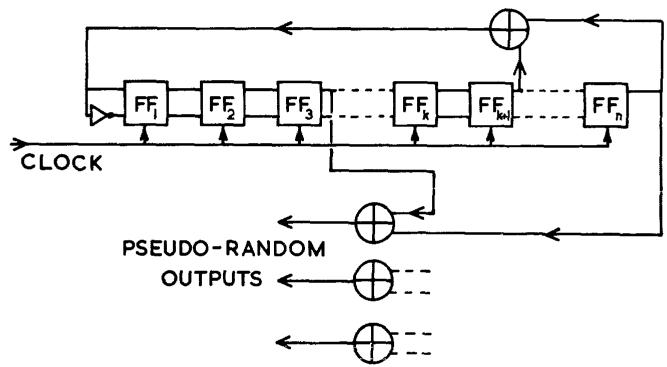
\includegraphics[keepaspectratio]{images/e461dd2b34742f61ee15e7f93e5f386678fa36ebbf7e38c1db4fface1c924d3e.jpg}}\\
Figure 11---Central pseudo-random generator

The Mark II Stochastic Computer, at present under construction, uses
entirely different techniques which have reduced both size and cost and
increased the clock-frequency to 1Mcs. A single, central pseudorandom
shift-register9,16 is used to generate stochastic

sequences for all computing elements. Different sequences for each
element are obtained by appropriate exclusive-OR gating of the
shift-register outputs, giving delayed replicas of the sequence in the
shift register itself. Such a generator is illustrated in Figure 11, and
with 43 flip-flops it is capable of supplying 100 16-bit integrators for
one hour without cross-duplication.

Serial arithmetic is used in the integrators of the Mark II computer so
that the counter may be realized using shift registers and the
comparators by far fewer gates. In this way a sixteen-bit stochastic
integrator may now be fabricated from only six dual in-line packages. A
clock-frequency of 16 Mcs in the shift-registers gives rise to a
clock-frequency of 1 Mcs in the stochastic computer, and respectable
bandwidths of 100 cs or so may now be attained.

\section{Applications of stochastic
computers}\label{applications-of-stochastic-computers}

The Stochastic Computer was developed for problems arising in automatic
control, and immediate applications are apparent mainly in the fields of
adaptive control and adaptive filtering. Gradient techniques for process
identification and on-line optimization are the simplest examples of
powerful control methods which lack the hardware necessary for their
full exploitation. Direct digital control using conventional computers
is not practical with a small plant, and conventional analog computers
are expensive because of the large numbers of multipliers required.
Two-level or polarity-coincidence multiplication10,11 has been
suggested12 as one means of realizing gradient techniques cheaply and
reliably using digital integrated circuits; however a comparison of six
techniques for multiplication in a steepest-descent computation has
shown that, for the same convergence-time, polarity-coincidence and
relay multiplication give much greater variance in parameter estimates
than does the equivalent stochastic-computing configuration.5 In this
particular computation the stochastic multiplier may be regarded as a
statistically-linearized13,14 polarity-coincidence multiplier, and the
addition of sawtooth dither to the input signals, which has been
suggested as a means of effecting such linearization,11,15,16 may be
seen as a technique for obtaining a pseudo-stochastic sequence.

Maximum likelihood prediction based on Bayes inversion of conditional
probabilities is the basis of many `learning machines' for control and
pattern-recognition, but the equations for estimation and prediction are
difficult to realize with conventional computing elements, and a
stored-program digital computer has been required for experiments with
this technique. Using a three-input variation of the ADDIE, however, the
estimation of normalized likelihood ratios, and pre

diction based on them, become very simple operations requiring little
hardware.5

The theoretical basis for the economy in hardware offered by stochastic
computing lies in a theorem of Rabin \(^{17}\) and Paz, \(^{18}\) to the
effect that a stochastic (or probabilistic) automaton is equivalent to a
deterministic automaton which generally has more states. An immediate
practical example of this phenomenon may be found in adaptive threshold
logic as used in pattern-classifiers such as the Perceptron \(^{19}\) or
Adaline. \(^{20}\) An adaptive threshold logic element with discrete
weights will not necessarily converge under the Novikoff conditions,
\(^{21}\) even though the weights can take values giving linear
separation, whilst the equivalent stochastic element may be shown to
converge under the same conditions. \(^{5}\)

A pictorial explanation of this difference is that the direction of
steepest descent followed in adaptive threshold logic with continuous
weights cannot be taken if the weights are discrete, and there are then
several directions of `almost steepest descent.' Deterministic logic has
to `chose' one of these directions and, if it is the `wrong' one, may
get into a cycle of wrong decisions, whereas stochastic logic has a
probability of taking any of the possible directions of descent and is
bound to take the right one eventually.

\section{CONCLUSION}\label{conclusion}

The main performance measure of a computer are size and range of
possible problems, speed and accuracy of solution, and physical size,
reliability and cost of the computer. There are strong interactions
between these measures and it is unlikely that any one form of computer
will ever be optimal on all counts. The identification and simulation of
complex processes, and the realization of multi-variable control
systems, requires large numbers of computing elements such as
multipliers, summers and integrators, working simultaneously and costing
little. However these elements do not have to compute a solution quickly
or accurately, for a bandwidth of 10 cs and an overall accuracy of
\(1\%\) is adequate in the simulation of economic and chemical
processes, and in control systems where feedback is operative a
computational accuracy of \(10\%\) may be ample. In these situations it
is advantageous to trade the accuracy of the digital computer and the
speed of the analog computer, for the economy of the stochastic
computer.

\section{ACKNOWLEDGMENTS}\label{acknowledgments}

My thanks are due to Dr.~J. H. Andreae (now at University of Canterbury,
Christchurch, N.Z.) for long discussions on learning machines and
computers, and for his criticism of this manuscript; to Mr.~P. L. Joyce

for constructing the first Stochastic Computer and obtaining the results
of Figure 9, and to S.T.L. for permission to publish this paper.

\section{REFERENCES}\label{references}

1 J. H. ANDREAE Learning machines in Encyclopaedia of Information,
Linguistics and Control (Pergamon Press, to be published)\\
2 B. R. GAINES and J. H. ANDREAE A learning machine in the context of
the general control problem Proceedings of the 3rd Congress of IFAC
1966\\
3 G. NAGY A survey of analog memory devices IEEE Trans. Electron. Comp.
12 388 1963\\
4 B. R. GAINES Stochastic computers in Encyclopaedia of Information,
Linguistics and Control Pergamon Press, to be published\\
5 B. R. GAINES Techniques of identification with the stochastic computer
Proc. IFAC Symp. Problems of Identification 1967\\
6 F. V. MAYOROV and Y. CHU Digital differential analysers IIiffe Books,
London 1964\\
7 H. SCHMID ``An operational hybrid computing system IEEE Trans.
Electron Comp. 12 715 1963\\
8 B. R. GAINES and P. L. JOYCE Phase computers 5th AICA Congress 1967\\
9 W. W. PETERSON Error correcting codes MIT Press \& Wiley, New York
1961\\
10 C. L. BECKER and J. V. WAIT Two-level correlation on an analog
computer IRE Trans. Electron Comp. 10 752 1961

11 B. P. TH. VELTMAN and A. van den BOS The applicability of the relay
correlator and the polarity coincidence correlator in automatic control
Proc. 2nd Congress IFAC 1963\\
12 P. EYKHOFF, P. M. van der GRINTEN, H. KWAKERNAAK, B. P. TH. VELTMAN
Systems modelling and identification Survey Paper 3rd Congress of IFAC
1966\\
13 O. I. ELGERD High frequency signal injection: a means of changing the
transfer characteristics of nonlinear elements WESCON 1962\\
14 A. A. PERVOZANSKII Random processes in nonlinear control Academic
Press, New York 1965\\
15 P. JESPERS, P. T. CHU, and A. FETTWEIS A new method to compute
correlation functions Proc. Int. Symp. Inf. Theo. 1962\\
16 G. A. KORN Random-process simulation and measurement McGraw Hill,
Inc.~1966\\
17 M. O. RABIN Probabilistic automata Inf. \& Contr. 6 230 1963\\
18 A. PAZ Some aspects of probabilistic automata Inf. \& Contr. 9 26
1966\\
19 F. ROSENBLATT A model for experimental storage in neural networks in
Computer and Information Sciences Spartan Books, Washington, D.C. 1964\\
20 B. WIDROW and F. W. SMITH Pattern-recognizing control systems in
Computer and Information Sciences Spartan Books, Washington, D.C. 1964\\
21 A. NOVIKOFF Convergence proofs for perceptrons in Mathematical Theory
of Automata Polytechnic Press, Brooklyn \& Wiley Interscience 1963

\end{document}
